\documentclass[11pt,openany]{report}

% ============================================================
%  preamble.tex -- qp pipeline technical documentation
%  Engine: pdflatex.  Build via latexmk (see Makefile).
% ============================================================

\usepackage[T1]{fontenc}
\usepackage[utf8]{inputenc}

\usepackage{amsmath}
\usepackage{amssymb}
\usepackage{newpxtext}
\usepackage{newpxmath}
\usepackage[scaled=0.96]{inconsolata}
\usepackage{microtype}

\usepackage[a4paper,margin=2.6cm,top=2.9cm,bottom=2.9cm]{geometry}
\usepackage{setspace}
\setstretch{1.06}

\usepackage{graphicx}
\usepackage{xcolor}
\usepackage{booktabs}
\usepackage{array}
\usepackage{tabularx}
\usepackage{longtable}
\usepackage{ragged2e}
\usepackage{enumitem}
\setlist{itemsep=2pt,topsep=3pt,parsep=0pt}
\usepackage{csquotes}
\usepackage[most]{tcolorbox}

\usepackage{tikz}
\usetikzlibrary{positioning,arrows.meta,shapes.geometric,fit,backgrounds,calc,chains}

\usepackage{listings}
\usepackage{url}

% ---------- palette (steel / signal-green, a trading-terminal feel) ----------
\definecolor{QpInk}{HTML}{16202B}
\definecolor{QpGrey}{HTML}{51606E}
\definecolor{QpSteel}{HTML}{2C5B73}
\definecolor{QpSteelDark}{HTML}{1E4152}
\definecolor{QpGreen}{HTML}{2E7D5B}
\definecolor{QpAmber}{HTML}{B07C2A}
\definecolor{QpRed}{HTML}{9C463C}
\definecolor{QpMist}{HTML}{ECEEF0}
\definecolor{QpLine}{HTML}{D6DADE}
\definecolor{QpCodeBg}{HTML}{101820}
\definecolor{QpCodeFg}{HTML}{DCE6E8}
\definecolor{QpCodeComment}{HTML}{7FA98E}
\definecolor{QpCodeKeyword}{HTML}{E8B168}
\definecolor{QpCodeString}{HTML}{9FC6D8}

% ---------- headings ----------
\usepackage{titlesec}
\titleformat{\chapter}[display]
  {\normalfont\huge\bfseries\color{QpSteelDark}}
  {\normalfont\Large\bfseries\color{QpAmber}\MakeUppercase{\chaptertitlename}\ \thechapter}
  {8pt}{\Huge}
\titlespacing*{\chapter}{0pt}{6pt}{28pt}
\titleformat{\section}
  {\normalfont\large\bfseries\color{QpSteelDark}}{\thesection}{0.8em}{}
\titleformat{\subsection}
  {\normalfont\normalsize\bfseries\color{QpInk}}{\thesubsection}{0.7em}{}

% ---------- headers / footers ----------
\usepackage{fancyhdr}
\pagestyle{fancy}
\fancyhf{}
\renewcommand{\headrulewidth}{0.4pt}
\renewcommand{\footrulewidth}{0pt}
\fancyhead[L]{\footnotesize\color{QpGrey}\nouppercase{\leftmark}}
\fancyhead[R]{\footnotesize\color{QpGrey}qp -- pipeline documentation}
\fancyfoot[C]{\thepage}
\fancypagestyle{plain}{\fancyhf{}\fancyfoot[C]{\thepage}\renewcommand{\headrulewidth}{0pt}}

% ---------- links ----------
\usepackage[hidelinks,breaklinks=true]{hyperref}
\hypersetup{
  colorlinks=true,
  linkcolor=QpSteelDark,
  citecolor=QpAmber,
  urlcolor=QpSteelDark,
  pdftitle={qp: A Systematic Trading Research Pipeline},
  pdfauthor={Batbandi Gerelkhuu}
}
\usepackage{bookmark}

% ---------- tables ----------
\newcolumntype{L}[1]{>{\RaggedRight\arraybackslash}p{#1}}
\newcolumntype{C}[1]{>{\Centering\arraybackslash}p{#1}}
\renewcommand{\arraystretch}{1.28}
\newcommand{\thh}[1]{\textbf{\textcolor{QpSteelDark}{#1}}}

% ---------- callouts ----------
\newtcolorbox{designnote}[1][]{
  enhanced, breakable, colback=QpMist, colframe=QpSteel,
  boxrule=0pt, leftrule=3pt, arc=1pt, left=10pt, right=10pt, top=8pt, bottom=8pt,
  fonttitle=\bfseries\color{QpSteelDark}, title={Design rationale}, #1 }

\newtcolorbox{caveat}[1][]{
  enhanced, breakable, colback=QpMist, colframe=QpRed,
  boxrule=0pt, leftrule=3pt, arc=1pt, left=10pt, right=10pt, top=8pt, bottom=8pt,
  fonttitle=\bfseries\color{QpRed}, title={Honest caveat}, #1 }

\newtcolorbox{cli}[1][]{
  enhanced, breakable, colback=QpCodeBg, colframe=QpCodeBg,
  arc=2pt, left=10pt, right=10pt, top=7pt, bottom=7pt,
  fontupper=\ttfamily\small\color{QpCodeFg}, #1 }

\newcommand{\keyline}[1]{%
  \par\vspace{4pt}{\itshape\color{QpSteelDark}#1}\par\vspace{4pt}}

% ---------- code listings (Python) ----------
\lstdefinestyle{qpy}{
  backgroundcolor=\color{QpCodeBg},
  basicstyle=\ttfamily\footnotesize\color{QpCodeFg},
  keywordstyle=\color{QpCodeKeyword}\bfseries,
  commentstyle=\color{QpCodeComment}\itshape,
  stringstyle=\color{QpCodeString},
  numbers=left, numberstyle=\tiny\color{QpGrey}, numbersep=8pt,
  breaklines=true, showstringspaces=false, tabsize=4,
  frame=none, xleftmargin=1.2em, framexleftmargin=1em,
  language=Python,
  columns=fullflexible,
  aboveskip=8pt, belowskip=8pt,
}
\lstset{style=qpy}

% ---------- tikz styles for architecture diagrams ----------
\tikzset{
  stage/.style={
    rectangle, rounded corners=2pt, draw=QpSteel, line width=0.8pt,
    fill=QpMist, text=QpInk, align=center, inner sep=7pt,
    font=\small\bfseries, minimum height=1.05cm, minimum width=2.6cm },
  stagealt/.style={
    rectangle, rounded corners=2pt, draw=QpAmber, line width=0.9pt,
    fill=QpAmber!12, text=QpInk, align=center, inner sep=7pt,
    font=\small\bfseries, minimum height=1.05cm, minimum width=2.6cm },
  flowarr/.style={-{Stealth[length=2.6mm]}, line width=0.9pt, draw=QpGrey },
  note/.style={ font=\scriptsize\itshape, text=QpGrey, align=center },
}


\title{\vspace{-1.5cm}
  {\color{QpAmber}\large\bfseries TECHNICAL DOCUMENTATION}\\[6pt]
  {\color{QpSteelDark}\Huge\bfseries qp: A Systematic Trading\\ Research Pipeline}\\[10pt]
  {\color{QpInk}\large Architecture, Design Rationale, and First Results}}
\author{Batbandi Gerelkhuu}
\date{Compiled 4 September 2026 \quad$\cdot$\quad v0.1.0}

\begin{document}

\pagenumbering{roman}
\maketitle
\thispagestyle{empty}

\begin{center}
\begin{minipage}{0.86\textwidth}
\small\itshape\color{QpGrey}
This document describes a research and paper-trading system, not a live trading
strategy. Every headline number in Chapter~8 is measured on synthetic data with
an injected, exaggerated signal so the machinery is visible end to end --- it is
not evidence that the included strategies make money on real markets. See
Chapter~10 for the caveats this document insists you read.
\end{minipage}
\end{center}

\vfill
\noindent\rule{\textwidth}{0.4pt}\\[2pt]
{\footnotesize\color{QpGrey}Repository: \texttt{quant-pipeline/} (sibling to the
Mongolia blueprint and the PyPSA thesis work). Code: \texttt{src/qp/}. Tests:
\texttt{tests/} (13 passing). Agent layer: \texttt{mcp/server.py}.}

\clearpage
\tableofcontents
\clearpage

\pagenumbering{arabic}

\chapter*{Executive Summary}
\addcontentsline{toc}{chapter}{Executive Summary}
\markboth{Executive Summary}{Executive Summary}

\texttt{qp} is a full systematic-trading research pipeline: configuration,
data ingestion, feature engineering, alpha signals, walk-forward validation,
a cost-aware vectorised backtester, pre-trade risk limits, a paper-trading
broker, reporting, and a live-loop orchestrator -- with a Model Context
Protocol (MCP) server on top so an agent can drive the whole thing. It is
roughly 2{,}400 lines of Python across 30 modules, has 13 passing tests, and
runs clean under \texttt{ruff}.

\section*{Why this exists}

Not to make money trading. Retail systematic trading is a near-zero-sum game
against firms with better data, lower fees, and colocation; Chapter~10 makes
that case in full. \texttt{qp} was built for two reasons instead:

\begin{enumerate}
  \item It is the portfolio artefact for an energy/commodity trading-desk
  application -- a clean backtester and a market model map directly onto what
  those roles actually do (Chapter~8 of the companion Mongolia blueprint;
  Part~I of this document shows the mechanics).
  \item It teaches market microstructure that compounds: no-look-ahead
  discipline, realistic transaction costs, walk-forward validation, and why an
  LSTM usually loses to a simple rule once costs are charged.
\end{enumerate}

\section*{What is in it}

\begin{table}[h]
\footnotesize
\centering
\begin{tabularx}{\textwidth}{L{2.6cm} X}
\toprule
\thh{Stage} & \thh{What it does} \\
\midrule
\texttt{config} & one YAML fully describes a run; typed \texttt{pydantic} models per stage \\
\texttt{data} & \texttt{DataSource} contract: synthetic (deterministic default), CSV, yfinance, stooq; parquet cache \\
\texttt{features} & causal technical indicators, token-resolved (\texttt{mom\_60}, \texttt{rsi\_14}); leak-free ML dataset builder \\
\texttt{signals} & momentum, mean-reversion, cross-sectional momentum, a walk-forward ML model, an optional LSTM \\
\texttt{validation} & walk-forward and purged $K$-fold splits with an embargo \\
\texttt{backtest} & vectorised, one-bar execution lag, $\sqrt{w^\top\Sigma w}$ vol targeting, full cost model \\
\texttt{risk} & per-name and gross exposure caps, a drawdown kill-switch with cooldown \\
\texttt{execution} & a JSON-persisted paper broker (default); a real-broker adapter left as a deliberate stub \\
\texttt{report} & a matplotlib tearsheet plus machine-readable metrics \\
\texttt{live} & the pull~$\to$~features~$\to$~signal~$\to$~target~$\to$~reconcile~$\to$~orders loop \\
\texttt{mcp} & the pipeline exposed as seven agent-callable tools \\
\bottomrule
\end{tabularx}
\end{table}

\section*{Headline result}

On the bundled synthetic demo, a simple cross-sectional momentum rule delivers
a Sharpe ratio of 0.62 after realistic costs; a gradient-boosted ML model on
the same data, engineered to look attractive, delivers roughly $-0.1$. That gap
is the point of this whole exercise, not an embarrassment: Chapter~8 shows the
numbers and Chapter~10 explains why it is the expected and correct outcome.

\chapter{System Architecture}

\section{The stage pipeline}

A run is one YAML file (\texttt{configs/*.yaml}) interpreted by a chain of
pure, testable stages. Each stage reads only the sub-model of \texttt{RunConfig}
it needs, so configs stay flat and reviewable, and each stage can be tested in
isolation with synthetic inputs.

\begin{figure}[h]
\centering
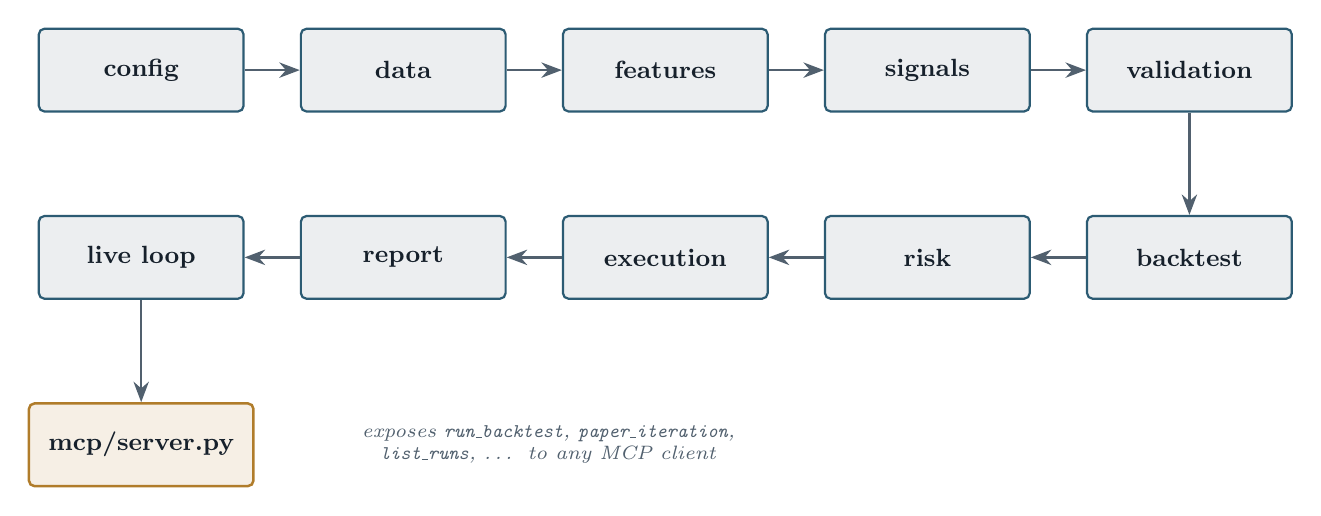
\begin{tikzpicture}[node distance=7mm]
  \node[stage] (cfg)  {config};
  \node[stage, right=of cfg]  (dat)  {data};
  \node[stage, right=of dat]  (feat) {features};
  \node[stage, right=of feat] (sig)  {signals};
  \node[stage, right=of sig]  (val)  {validation};
  \draw[flowarr] (cfg)--(dat); \draw[flowarr] (dat)--(feat);
  \draw[flowarr] (feat)--(sig); \draw[flowarr] (sig)--(val);

  \node[stage, below=13mm of val] (bt)   {backtest};
  \node[stage, left=of bt]  (risk) {risk};
  \node[stage, left=of risk] (exec) {execution};
  \node[stage, left=of exec] (rep)  {report};
  \node[stage, left=of rep]  (live) {live loop};
  \draw[flowarr] (val.south) -- (bt.north);
  \draw[flowarr] (bt)--(risk); \draw[flowarr] (risk)--(exec);
  \draw[flowarr] (exec)--(rep); \draw[flowarr] (rep)--(live);

  \node[stagealt, below=13mm of live] (mcp) {mcp/server.py};
  \draw[flowarr] (live.south) -- (mcp.north);
  \node[note, right=4mm of mcp, text width=6.4cm] {exposes \texttt{run\_backtest},
    \texttt{paper\_iteration}, \texttt{list\_runs}, \ldots{} to any MCP client};
\end{tikzpicture}
\caption{The eleven modules of \texttt{src/qp/}, in call order. The bottom row
reads right to left to keep the diagram compact; data still flows
backtest~$\to$~risk~$\to$~execution~$\to$~report~$\to$~live.}
\end{figure}

\section{Orchestration}

\texttt{qp.pipeline.run\_pipeline(cfg)} is the single entry point used by the
CLI's \texttt{demo} and \texttt{backtest} commands:

\begin{lstlisting}
long_df = load_prices(cfg.data)                  # data
close   = to_wide(long_df, "close")
signal  = make_signal(cfg.signal, cfg.features, cfg.validation)
scores  = signal.generate(close)                 # features + signals (fused)
result  = run_backtest(close, scores, cfg)        # validation + backtest + risk
write_tearsheet(result, cfg.run_dir())           # report
\end{lstlisting}

\texttt{qp.live.loop.run\_once(cfg)} reuses the same \texttt{data}, \texttt{features},
and \texttt{signals} code, then diverges into \texttt{execution} instead of
\texttt{backtest} -- the live loop and the backtester are guaranteed to compute
the same target weights from the same signal, because they call the same
functions.

\section{Why this shape}

\begin{designnote}
Every stage is a pure function or a small class with one public method
(\texttt{generate}, \texttt{fetch}, \texttt{rebalance\_to}). Nothing reaches into
another stage's internals. That buys three things directly relevant to career
capital: (1) each stage is unit-testable against synthetic data without a
network or a broker; (2) a new signal, data source, or broker is additive, not
a rewrite; (3) the same code path serves the backtester and the live loop, so
there is no ``it worked in backtest but not live'' class of bug from divergent
implementations.
\end{designnote}

\chapter{The Data Layer}

\section{Contract}

Every source implements \texttt{DataSource.fetch(symbols, start, end) -\/> DataFrame}
and returns a long OHLCV frame validated against one schema:

\begin{table}[h]
\footnotesize
\centering
\begin{tabularx}{\textwidth}{L{2.2cm} X}
\toprule
\thh{Column} & \thh{Meaning} \\
\midrule
\texttt{date} & trading date (parsed to \texttt{datetime64}) \\
\texttt{symbol} & instrument identifier \\
\texttt{open, high, low, close} & prices; \texttt{close} is adjusted where the source provides it \\
\texttt{volume} & traded volume \\
\bottomrule
\end{tabularx}
\end{table}

\texttt{DataSource.\_validate} enforces the schema, sorts by \texttt{(symbol, date)},
and rejects non-positive prices before any downstream code sees the frame.
\texttt{qp.data.store.load\_prices} wraps a source with a content-addressed
parquet cache: the config's data section is hashed, and a repeat run with an
identical configuration reads from disk instead of re-fetching.

\section{Four sources, one always working}

\begin{table}[h]
\footnotesize
\centering
\begin{tabularx}{\textwidth}{L{2.6cm} X}
\toprule
\thh{Source} & \thh{Notes} \\
\midrule
\texttt{synthetic} & default; zero dependencies, zero network, deterministic given a seed. Used by every test and the demo. \\
\texttt{csv} & one file per symbol under \texttt{data.csv\_dir}; the robust path for real historical data (e.g.\ an ENTSO-E export). \\
\texttt{yfinance} & guarded optional import (\texttt{pip install "qp[data]"}); degrades to a clear \texttt{ImportError} rather than a broken run. \\
\texttt{stooq} & stdlib-only HTTP fetch; best-effort, since stooq's endpoint has started serving a bot-check page from some networks. \\
\bottomrule
\end{tabularx}
\caption{The pipeline never depends on network access to run its tests or its demo.}
\end{table}

\section{The synthetic generator}

Real market data cannot be committed to a repository and real free APIs are
unreliable enough to break a demo. \texttt{qp.data.synthetic.SyntheticSource}
solves both problems and, deliberately, does one more job: it injects a
\emph{known, controllable} amount of predictable structure so the rest of the
pipeline has something real to find.

For $k$ symbols over $n$ trading days, log-returns follow a correlated
geometric Brownian motion with a slow-moving, per-symbol drift component:

\begin{align}
  r_t &= \left(\mu_t + \alpha_t - \tfrac{1}{2}\sigma_t^2\right)\Delta t
         + \sigma_t \sqrt{\Delta t}\; L\, z_t, \qquad z_t \sim \mathcal N(0, I_k) \\
  \alpha_t &= \phi\, \alpha_{t-1} + \varepsilon_t, \qquad \varepsilon_t \sim \mathcal N(0, \eta^2 I_k)
\end{align}

where $\Delta t = 1/252$, $L$ is the Cholesky factor of a correlation matrix
with off-diagonal $\rho$ (a one-factor structure: every pair of symbols shares
correlation $\rho$), and $(\mu_t, \sigma_t)$ follow a regime path that switches
between hand-tuned \emph{bull}, \emph{bear}, and \emph{chop} states (durations
drawn from $\mathcal N(\text{mean length}, 0.25\cdot\text{mean length})$, floored
at 20 days). $\alpha_t$ is an AR(1) process per symbol with $\phi = 0.99$
(half-life $\approx 69$ trading days) -- the only genuinely forecastable
structure in the data, and the reason a momentum or ML signal has anything real
to capture. OHLC and volume are then simulated around each simulated close with
independent intraday noise.

\begin{table}[h]
\footnotesize
\centering
\begin{tabularx}{\textwidth}{L{3cm} X}
\toprule
\thh{Parameter} & \thh{Demo value} \\
\midrule
$\mu$ (baseline drift) & 6\%/year, regime-modulated \\
$\sigma$ (baseline vol) & 20\%/year, regime-modulated \\
$\rho$ (pairwise correlation) & 0.3 \\
$\phi$ (alpha persistence) & 0.99 \\
$\eta$, alpha scale & 0.08 innovation std, $\times 0.22$ overall \\
\bottomrule
\end{tabularx}
\caption{\texttt{configs/demo.yaml -> data.synthetic}. Every value is a config
knob; \texttt{qp demo} fixes them to produce a reproducible Sharpe~0.62 for
cross-sectional momentum (Chapter~8).}
\end{table}

\begin{caveat}
The alpha scale (0.22) is chosen so the demo is legible, not because it
resembles a real single-name equity anomaly. A genuine, persistent,
easily-captured 69-day alpha of this magnitude does not exist in liquid public
markets; if it did, it would already be arbitraged away. Treat every number in
Chapter~8 as a statement about the code, not about markets.
\end{caveat}

\chapter{Feature Engineering}

\section{Causal, token-resolved indicators}

Every function in \texttt{qp.features.technical} takes a wide close panel
(index = date, columns = symbol) and returns a same-shaped panel where row $t$
depends only on data up to and including $t$ -- there is no indicator in this
module that can see the future.

\begin{table}[h]
\footnotesize
\centering
\begin{tabularx}{\textwidth}{L{2.2cm} L{2.6cm} X}
\toprule
\thh{Token} & \thh{Formula} & \thh{Reads} \\
\midrule
\texttt{ret\_n} & $\ln P_t - \ln P_{t-n}$ & $n$-day log return \\
\texttt{vol\_n} & $\mathrm{std}_n(\Delta \ln P)\sqrt{252}$ & annualised realised volatility \\
\texttt{mom\_n} & $P_{t-\text{skip}}/P_{t-n-\text{skip}} - 1$ & trailing return, skipping the most recent \texttt{skip} days (avoids the well-known 1-week reversal contaminating a momentum signal) \\
\texttt{zscore\_n} & $(P_t - \mathrm{MA}_n)/\mathrm{SD}_n$ & distance from the rolling mean, in standard deviations \\
\texttt{rsi\_n} & $100 - 100/(1+RS)$, $RS = \overline{\Delta^+}_n / \overline{\Delta^-}_n$ & Wilder's relative strength index \\
\texttt{macd} & $\mathrm{EMA}_{12} - \mathrm{EMA}_{26}$, minus its own 9-day EMA & MACD histogram \\
\texttt{bbp\_n} & $(P_t - L_n)/(U_n - L_n)$, $U/L = \mathrm{MA}_n \pm 2\,\mathrm{SD}_n$ & \%B: position within the Bollinger band \\
\texttt{skew\_n} & rolling skewness of log-returns & tail asymmetry \\
\bottomrule
\end{tabularx}
\caption{Token grammar: \texttt{"<base>\_<window>"} resolves via a small registry
in \texttt{compute()}; a config just lists tokens like \texttt{mom\_60, rsi\_14}.}
\end{table}

\section{Building an ML dataset without leaking the future}

\texttt{build\_ml\_dataset(close, tokens, horizon)} produces a tidy
$(X, y)$ pair indexed by \texttt{(date, symbol)}:

\begin{lstlisting}
fwd = close.shift(-horizon) / close - 1.0   # row t: return realised over (t, t+horizon]
y   = fwd.stack()
X   = pd.concat([compute(tok, close).stack() for tok in tokens], axis=1)
df  = X.join(y, how="inner").dropna()
\end{lstlisting}

Two guarantees follow directly from this construction and are exercised by
\texttt{tests/test\_data\_features.py::test\_ml\_dataset\_no\_leakage}:

\begin{enumerate}
  \item every feature at row $(t, s)$ is computable from data available at the
  close of day $t$;
  \item the label at row $(t, s)$ is a \emph{forward} return, so the final
  \texttt{horizon} dates in the sample have no label and are dropped -- a model
  trained on this frame cannot see its own target.
\end{enumerate}

\begin{designnote}
The no-leakage property is enforced structurally (by the shift and the inner
join), not by convention or a code-review checklist. This is the single most
common way a backtest lies to its author, so it is worth making impossible
rather than merely discouraged.
\end{designnote}

\chapter{Signal Models}

\section{The contract}

Every signal implements \texttt{generate(close) -\/> DataFrame} of scores, same
shape as \texttt{close}. A score is a ``desire to hold'' in roughly $[-1, 1]$;
the portfolio layer (Chapter~6) turns scores into leverage- and risk-constrained
weights. A signal marks itself \texttt{market\_neutral = True} when it already
produces cross-sectionally demeaned scores.

\section{Rule-based signals}

\begin{table}[h]
\footnotesize
\centering
\begin{tabularx}{\textwidth}{L{3.4cm} X}
\toprule
\thh{Signal} & \thh{Score} \\
\midrule
\texttt{Momentum} & $\tanh\!\big(\mathrm{mom}_n / \overline{|\mathrm{mom}_n|}_{252}\big)$, optionally divided by realised vol so noisier names are sized down \\
\texttt{MeanReversion} & $-z_n / (2\cdot\text{entry\_z})$, clipped to $[-1,1]$: fade a stretched short-horizon z-score \\
\texttt{CrossSectionalMomentum} & cross-sectional z-score of $\mathrm{mom}_n$, renormalised each day so $\sum_s |w_s| \approx 1$: long the relative winners, short the relative losers, market-neutral \\
\bottomrule
\end{tabularx}
\end{table}

\texttt{CrossSectionalMomentum} is the pipeline's default and the one used for
the headline demo result -- it is the closest rule-based analogue of the
persistent per-symbol $\alpha_t$ injected into the synthetic data (Chapter~2),
so it is the fairest baseline for the ML comparison in Chapter~8.

\section{A walk-forward ML signal}

\texttt{MLSignal} wraps a \texttt{scikit-learn} pipeline
(\texttt{StandardScaler} + \texttt{HistGradientBoostingRegressor} by default) and
trains it \emph{only} on the walk-forward splits described in Chapter~5: for
each \texttt{(train\_start, train\_end, test\_start, test\_end)} window it fits
on the training rows of the leak-free dataset from Chapter~3, predicts on the
test rows, and stitches the out-of-sample predictions back into a wide panel.
The cross-sectional z-score of that prediction becomes the score, exactly as in
\texttt{CrossSectionalMomentum} -- so the two signals are compared on equal
footing in Chapter~8: same sizing, same costs, same risk limits, different
alpha source.

\section{An optional sequence model}

\texttt{SequenceSignal} is a single-layer LSTM over a rolling window of the same
feature tokens, trained walk-forward with the same split logic:

\begin{figure}[h]
\centering
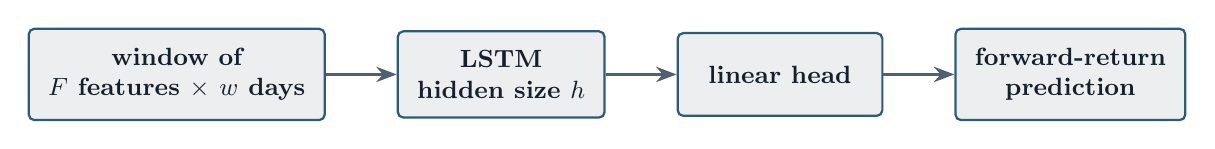
\begin{tikzpicture}[node distance=9mm]
  \node[stage] (in) {window of \\ $F$ features $\times$ $w$ days};
  \node[stage, right=of in] (lstm) {LSTM \\ hidden size $h$};
  \node[stage, right=of lstm] (head) {linear head};
  \node[stage, right=of head] (out) {forward-return \\ prediction};
  \draw[flowarr] (in)--(lstm); \draw[flowarr] (lstm)--(head); \draw[flowarr] (head)--(out);
\end{tikzpicture}
\caption{One (symbol, date) training example: the last $w$ days of the feature
panel for that symbol, target = forward return over \texttt{horizon} days. The
final hidden state feeds a linear head; only the last time step's output is
used (\texttt{out[:, -1, :]}).}
\end{figure}

It requires \texttt{torch} and is import-guarded: without the \texttt{ml} extra
installed, selecting \texttt{signal.type: sequence} raises a clear
\texttt{ImportError} naming the alternatives, rather than crashing deep inside a
training loop.

\begin{caveat}
This is included to \emph{learn the architecture and benchmark it honestly},
not because it is expected to win. Chapter~10 explains why an LSTM over
technical features is dominated by transaction costs and regime shift on real
data far more often than it earns its keep. Never trust a sequence model's
in-sample equity curve.
\end{caveat}

\chapter{Validation Methodology}

Standard $K$-fold cross-validation assumes exchangeable, independent samples.
Financial time series are neither: adjacent rows overlap (a 5-day forward
return at $t$ and at $t+1$ share four days of data), so a naive random split
leaks the future into the training set through that overlap. \texttt{qp.validation}
implements two splitters that respect time ordering and remove the overlap.

\section{Walk-forward}

\begin{figure}[h]
\centering
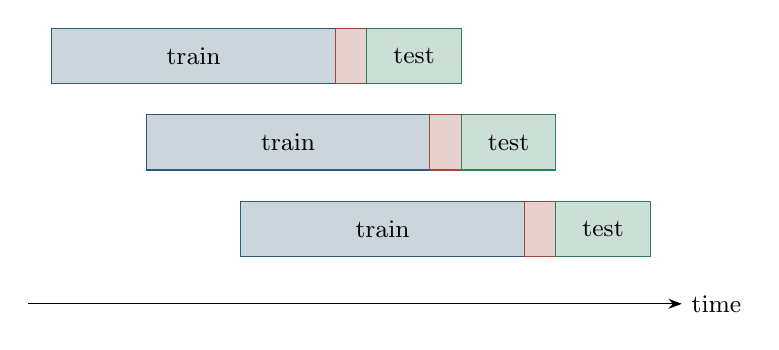
\begin{tikzpicture}[node distance=2mm]
  \foreach \x/\lbl/\col in {0/train/QpSteel, 3.6/embargo/QpRed, 4.1/test/QpGreen} {}
  \draw[fill=QpSteel!25, draw=QpSteel] (0,0) rectangle (3.6,0.7) node[midway]{\small train};
  \draw[fill=QpRed!25, draw=QpRed] (3.6,0) rectangle (4.0,0.7);
  \draw[fill=QpGreen!25, draw=QpGreen] (4.0,0) rectangle (5.2,0.7) node[midway]{\small test};

  \draw[fill=QpSteel!25, draw=QpSteel] (1.2,-1.1) rectangle (4.8,-0.4) node[midway]{\small train};
  \draw[fill=QpRed!25, draw=QpRed] (4.8,-1.1) rectangle (5.2,-0.4);
  \draw[fill=QpGreen!25, draw=QpGreen] (5.2,-1.1) rectangle (6.4,-0.4) node[midway]{\small test};

  \draw[fill=QpSteel!25, draw=QpSteel] (2.4,-2.2) rectangle (6.0,-1.5) node[midway]{\small train};
  \draw[fill=QpRed!25, draw=QpRed] (6.0,-2.2) rectangle (6.4,-1.5);
  \draw[fill=QpGreen!25, draw=QpGreen] (6.4,-2.2) rectangle (7.6,-1.5) node[midway]{\small test};

  \draw[-{Stealth}] (-0.3,-2.8) -- (8.0,-2.8) node[right]{\small time};
\end{tikzpicture}
\caption{\texttt{walk\_forward(dates, train\_days, test\_days, step\_days, embargo\_days)}.
The window slides forward by \texttt{step\_days} each iteration; the red embargo
gap between train and test is at least as long as the label horizon, so no
training row's label overlaps a test-period date.}
\end{figure}

\texttt{MLSignal} and \texttt{SequenceSignal} both consume this splitter directly.
For each window they train fresh (no state carried across windows -- a
deliberate choice: it exercises the model's ability to relearn from only recent
regime data, which is closer to how a live system would operate) and predict
on the test window only; the concatenation of all test predictions is the
out-of-sample score series used everywhere downstream.

\section{Purged $K$-fold}

\texttt{purged\_kfold(dates, n\_splits, embargo\_days)} implements the
Lopez-de-Prado-style alternative: split the date range into $K$ contiguous test
folds, and for each fold drop every training row within \texttt{embargo\_days}
of that fold's boundary on either side. This is available for parameter
studies where multiple folds are needed cheaply; the pipeline's default
(\texttt{validation.scheme: walk\_forward}) is the more realistic choice for
anything that will inform a live decision, because it never trains on data from
after the period it is being evaluated on -- purged $K$-fold's later folds can
still train on data that is chronologically after an earlier test fold, which
walk-forward never does.

\begin{designnote}
The embargo is not cosmetic. With a 5-day forward-return target and no embargo,
a model can partially ``see'' test-period information through overlapping
labels at the train/test boundary -- a subtle leak that inflates backtested
Sharpe without ever showing up as an obvious bug. Setting
\texttt{embargo\_days} $\geq$ the label horizon closes it structurally.
\end{designnote}

\chapter{The Backtest Engine}

\section{Timeline convention}

The single most common source of an inflated backtest is look-ahead: using
information at bar $t$ that would not actually have been known at bar $t$. The
engine enforces one convention everywhere:

\begin{enumerate}
  \item scores and target weights for bar $t$ are computed from data available
  \emph{at the close} of bar $t$;
  \item those weights are \emph{held over} $t \to t+1$ (a one-bar execution lag:
  \texttt{held = target\_w.shift(1)});
  \item realised return over that bar is \texttt{held * asset\_return}, i.e.\
  yesterday's decision earns today's return, never today's decision earning
  today's return.
\end{enumerate}

\texttt{tests/test\_backtest.py::test\_no\_lookahead\_one\_bar\_lag} encodes this
as a unit test: a score that only exists on the final bar of the sample can
have no effect on that bar's return, because there is no bar $t+1$ to hold it
into.

\section{Position sizing}

Three sizing schemes share one pipeline: build raw scores, cap per name, project
to long-only if configured, then renormalise to the target gross leverage.

\paragraph{Fixed.} Weights proportional to score, renormalised to
\texttt{gross\_leverage}. No volatility adjustment.

\paragraph{Risk parity.} $w_s \propto \mathrm{sign}(\text{score}_s)/\sigma_s$
before the same renormalisation -- equal risk contribution per name under the
(strong) assumption of no cross-correlation.

\paragraph{Volatility targeting.} The book is scaled each day so its
\emph{ex-ante} volatility tracks a target:

\begin{equation}
  \sigma_{\text{port},t} = \sqrt{w_t^\top \Sigma_t\, w_t}\,\sqrt{252},
  \qquad
  w_t \leftarrow w_t \cdot \min\!\left(\frac{\sigma_{\text{target}}}{\sigma_{\text{port},t}},\; \kappa_{\max}\right)
\end{equation}

where $\Sigma_t$ is a rolling sample covariance of daily returns
(\texttt{vol\_lookback} days) and $\kappa_{\max}$
(\texttt{max\_leverage\_scale}) caps the multiplier so a quiet-market estimate
of $\Sigma_t$ cannot imply arbitrary leverage. This is computed from the
\emph{portfolio} covariance, not a sum of individual-name volatilities --
it therefore correctly rewards diversification and long/short netting: a
market-neutral book with two highly correlated offsetting legs is recognised
as low-risk, which a naive $\sum_s |w_s|\sigma_s$ proxy would not capture.

\begin{table}[h]
\footnotesize
\centering
\begin{tabularx}{\textwidth}{L{4.4cm} X}
\toprule
\thh{Config knob} & \thh{Effect} \\
\midrule
\texttt{target\_vol} & annualised target for $\sigma_{\text{port}}$ \\
\texttt{max\_weight} & per-name cap, applied before and after vol scaling \\
\texttt{gross\_leverage} & the leverage the raw (pre-vol-scale) book normalises to \\
\texttt{vol\_lookback} & window for $\Sigma_t$ \\
\texttt{max\_leverage\_scale} & ceiling on the vol-target multiplier $\kappa$ \\
\texttt{rebalance} & \texttt{daily} / \texttt{weekly} / \texttt{monthly}; weights hold between rebalance dates \\
\bottomrule
\end{tabularx}
\end{table}

\section{Cost model}

Turnover is the $L^1$ change in \emph{target} weight between consecutive bars,
$\tau_t = \sum_s |w_{s,t} - w_{s,t-1}|$. Costs charged against gross return:

\begin{align}
  \text{transaction cost}_t &= \tau_t \times \frac{\text{commission}_{\text{bps}} + \text{spread}_{\text{bps}} + \text{slippage}_{\text{bps}}}{10^4} \\
  \text{borrow cost}_t &= \Big(\sum_{s:\, w_{s,t}<0} |w_{s,t}|\Big) \times \frac{\text{borrow}_{\text{bps/yr}}}{10^4 \times 252}
\end{align}

Net return is \texttt{gross - transaction\_cost - borrow\_cost}. The tearsheet
(Chapter~7) plots the cumulative decomposition of all three terms so a
strategy's apparent edge can be checked against how much of it costs eat.

\section{Risk limits and the drawdown kill-switch}

Pre-trade, \texttt{risk.limits.apply\_limits} clips each name to
\texttt{max\_position} and rescales the whole book if gross exposure exceeds
\texttt{max\_gross}. Separately, the engine runs a drawdown kill-switch on the
realised net-return series:

\begin{quote}
\small\ttfamily
track running equity and its peak; the moment drawdown breaches
\texttt{max\_drawdown\_stop}, flatten the book (zero return, zero weight) for a
fixed \texttt{cooldown} (21 trading days by default); reset the peak on resume.
\end{quote}

This models a real risk desk's behaviour more faithfully than an instantaneous
recovery rule would: after a real stop-out, a desk does not resume risk the
instant equity happens to tick back up -- it sits out a cooldown period and
restarts clean.

\section{Metrics}

\texttt{qp.backtest.metrics.summary} reports, from the daily net-return series
$r_t$ (252 trading days/year):

\begin{align*}
  \text{CAGR} &= \Big(\textstyle\prod_t (1+r_t)\Big)^{252/N} - 1
  &\text{Sharpe} &= \sqrt{252}\,\dfrac{\overline{r_t - r_f/252}}{\mathrm{sd}(r_t - r_f/252)} \\
  \text{Sortino} &= \sqrt{252}\,\dfrac{\overline{r_t - r_f/252}}{\mathrm{sd}\big((r_t-r_f/252)^-\big)}
  &\text{Calmar} &= \dfrac{\text{CAGR}}{|\text{max drawdown}|} \\
  \text{VaR}_{95} &= Q_{0.05}(r_t)
  &\text{CVaR}_{95} &= \mathbb E[r_t \mid r_t \le \text{VaR}_{95}]
\end{align*}

plus hit rate, skew, kurtosis, best/worst day, and -- when a weights panel is
supplied -- average gross/net exposure, average daily turnover, and time in
market. This is the same dictionary written to \texttt{metrics.json} for every
run and read back by the MCP \texttt{list\_runs} tool (Chapter~9).

\chapter{Execution and the Live Loop}

\section{The broker contract}

\texttt{qp.execution.base.Broker} is four methods: \texttt{equity()},
\texttt{positions()}, \texttt{mark(prices)}, \texttt{rebalance\_to(target\_weights, prices)}.
The live loop only ever thinks in target weights; a broker implementation is
responsible for turning a weight vector into orders against its own current
positions.

\section{The paper broker}

\texttt{PaperBroker} is the default and, at this stage of the project, the only
broker that actually works. It holds cash and per-symbol share quantities in
memory, fills at the supplied price plus a symmetric slippage in basis points,
charges a commission, and -- critically -- persists its full state
(\texttt{cash}, \texttt{positions}, \texttt{last\_prices}, the last 500 fills) to
\texttt{execution\_state/<name>.json} after every rebalance:

\begin{lstlisting}
target_qty = (weight * equity) / price
delta      = target_qty - current_qty
fill_price = price * (1 + sign(delta) * slippage_bps / 1e4)
commission = abs(delta * fill_price) * commission_bps / 1e4
cash      -= delta * fill_price + commission
\end{lstlisting}

Because state is persisted, a fresh \texttt{PaperBroker(name=...)} constructed
later -- in a new process, after a reboot, from a cron job -- resumes exactly
where the last one left off. \texttt{tests/test\_pipeline\_exec.py::test\_paper\_broker\_rebalance\_and\_resume}
exercises this directly: two independently constructed broker instances sharing
a state directory see the same equity.

\section{The live loop}

\begin{figure}[h]
\centering
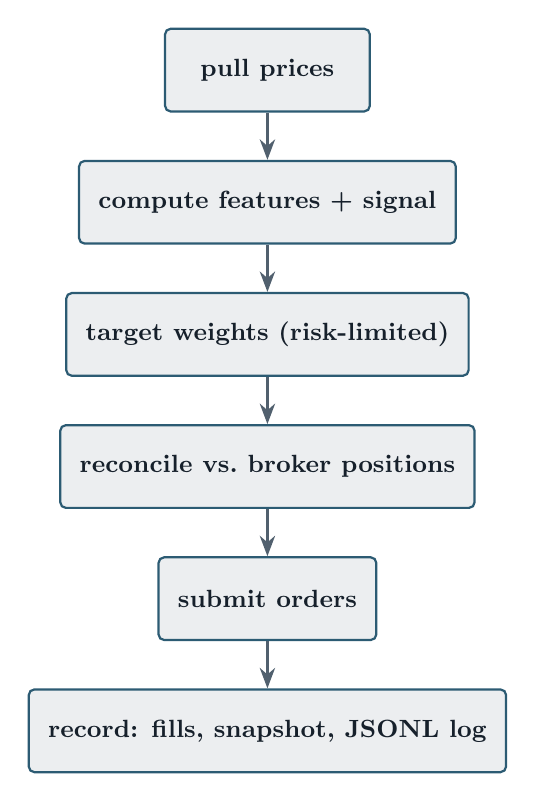
\begin{tikzpicture}[node distance=6mm]
  \node[stage] (a) {pull prices};
  \node[stage, below=of a] (b) {compute features + signal};
  \node[stage, below=of b] (c) {target weights (risk-limited)};
  \node[stage, below=of c] (d) {reconcile vs.\ broker positions};
  \node[stage, below=of d] (e) {submit orders};
  \node[stage, below=of e] (f) {record: fills, snapshot, JSONL log};
  \draw[flowarr] (a)--(b); \draw[flowarr] (b)--(c); \draw[flowarr] (c)--(d);
  \draw[flowarr] (d)--(e); \draw[flowarr] (e)--(f);
\end{tikzpicture}
\caption{\texttt{qp.live.loop.run\_once(cfg)}. Safe to call from cron:
each call is a self-contained iteration that ends by writing one JSON line to
\texttt{execution\_state/<name>.loop.jsonl} and the broker's own state file.
\texttt{run\_forever} is a thin \texttt{time.sleep} wrapper around the same
function for a long-running process.}
\end{figure}

The loop reuses the exact \texttt{load\_prices} / \texttt{make\_signal} /
\texttt{build\_weights} / \texttt{apply\_limits} functions the backtester uses
(Chapter~1) -- there is one implementation of ``turn a signal into a target
book,'' not two that could silently diverge.

\section{The real-broker stub}

\texttt{execution/alpaca.py} exists and raises \texttt{NotImplementedError} on
construction, with the wiring instructions in its docstring. This is deliberate,
not an oversight: the point at which paper trading has produced months of
consistent, believable results is the point at which wiring a live broker is a
conscious decision, not an accident of a config flag left on the wrong value.
Every bundled config defaults to \texttt{execution.broker: paper}.

\chapter{Results on the Bundled Demo}

Reproduce every number in this chapter with:

\begin{cli}
qp demo\\
qp walkforward -c configs/demo.yaml
\end{cli}

\section{The demo run}

\texttt{configs/demo.yaml}: 8 synthetic symbols, 2013--2024, \texttt{cross\_sectional\_momentum}
(60-day lookback, 5-day skip), volatility-targeted at 10\%/year, weekly
rebalance, 1\,bp commission + 2\,bp spread + 50\,bp/year borrow.

\begin{table}[h]
\footnotesize
\centering
\begin{tabularx}{\textwidth}{L{4.2cm} X L{4.2cm} X}
\toprule
\thh{Metric} & \thh{Value} & \thh{Metric} & \thh{Value} \\
\midrule
Trading days & 3{,}131 & Hit rate & 50.7\% \\
CAGR & 4.57\% & Skew / kurtosis & 0.08 / 2.87 \\
Annualised vol & 7.73\% & Daily VaR$_{95}$ / CVaR$_{95}$ & $-0.74\%$ / $-1.07\%$ \\
Sharpe & 0.62 & Avg.\ gross / net exposure & 1.34 / $-0.03$ \\
Sortino & 0.92 & Avg.\ daily turnover & 0.10 \\
Max drawdown & $-14.87\%$ & Time in market & 97.8\% \\
Calmar & 0.31 & & \\
\bottomrule
\end{tabularx}
\caption{\texttt{runs/demo/metrics.json}, reproduced exactly by \texttt{qp demo}
(fixed seed). Net exposure near zero confirms the book is running
market-neutral, as \texttt{CrossSectionalMomentum} is designed to.}
\end{table}

\begin{figure}[h]
\centering
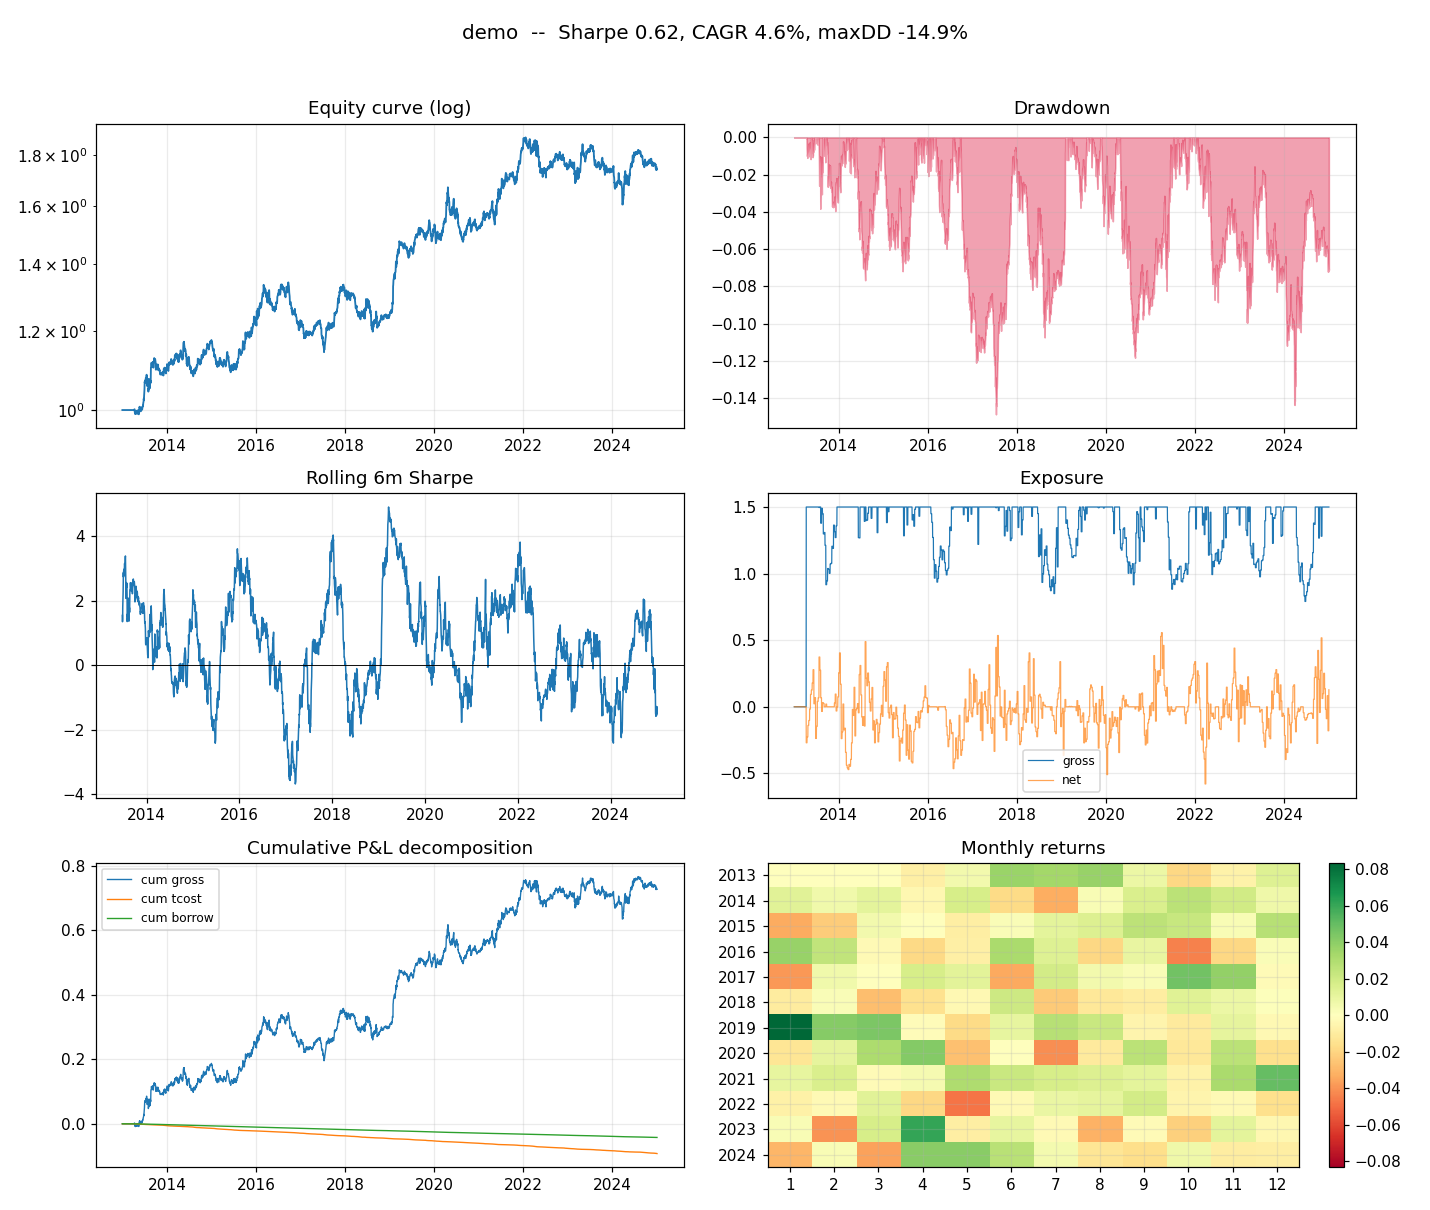
\includegraphics[width=\textwidth]{figures/tearsheet.png}
\caption{\texttt{runs/demo/tearsheet.png}: equity curve, drawdown, rolling
6-month Sharpe, gross/net exposure, cumulative P\&L decomposition (gross vs.\
transaction cost vs.\ borrow cost), and the monthly-return heatmap.}
\end{figure}

\section{Rule versus ML, same data, same costs}

\texttt{qp walkforward} runs \texttt{cross\_sectional\_momentum} and the
walk-forward \texttt{MLSignal} (a \texttt{HistGradientBoostingRegressor} on the
same feature set, 5-day forward-return target) through the identical sizing,
cost, and risk pipeline, on the identical dataset:

\begin{table}[h]
\footnotesize
\centering
\begin{tabularx}{\textwidth}{L{4cm} C{2.2cm} C{2.2cm} C{2.6cm} X}
\toprule
\thh{Variant} & \thh{Sharpe} & \thh{CAGR} & \thh{Max drawdown} & \thh{Avg.\ daily turnover} \\
\midrule
\texttt{cs\_momentum} & \textbf{0.62} & 4.6\% & $-14.9\%$ & 0.10 \\
\texttt{ml\_gbr} & $-0.07$ & $-0.7\%$ & $-21.1\%$ & 0.17 \\
\bottomrule
\end{tabularx}
\caption{Same universe, same walk-forward discipline, same cost model. The
simple rule wins, and by a wide margin.}
\end{table}

A second, independent dataset (\texttt{configs/ml\_walkforward.yaml} --
10 years, 8 different synthetic symbols, a fresh seed) gives the ML signal
Sharpe $-0.57$ on its own -- consistent with the comparison above, not a fluke
of one run.

\section{Why the rule beat the model here}

The synthetic alpha (Chapter~2) is a slow AR(1) process with a $\approx$69-day
half-life. A 60-day trailing-return momentum signal is close to a matched
filter for exactly that process. The ML model is asked to recover the same
signal from a 5-day-ahead target through a gradient-boosted tree over noisy
technical features -- a much harder estimation problem, with far more ways for
the model to fit noise in the training window that does not repeat in the test
window. This is not a defect in the implementation; it is the expected outcome
whenever a flexible model is pointed at a low signal-to-noise, slowly-varying
target without a structural reason to expect it to generalise better than a
simple, correctly-shaped rule. See Chapter~10 for the general version of this
argument and its implications for real markets.

\chapter{The Agent Layer: MCP, and What's Next}

\section{Why an MCP server on top of a CLI}

The CLI (\texttt{qp demo}, \texttt{qp backtest}, \texttt{qp walkforward}, \texttt{qp
paper}) is sufficient for a human at a terminal. An agent needs the same
capabilities as typed, discoverable tool calls rather than a stream of shell
output to parse -- and once the pipeline speaks MCP, it is reachable from
Claude Code, Claude Desktop, or any other MCP client (including, per the brief
this project started from, an orchestration layer like Google Stitch) without
writing a second integration.

\section{What is exposed today}

\begin{table}[h]
\footnotesize
\centering
\begin{tabularx}{\textwidth}{L{4.6cm} X L{2.6cm}}
\toprule
\thh{Tool} & \thh{Effect} & \thh{Side effects} \\
\midrule
\texttt{describe\_pipeline()} & returns this project's README & none \\
\texttt{list\_configs()} & lists \texttt{configs/*.yaml} & none \\
\texttt{list\_runs()} & lists \texttt{runs/*} with Sharpe/CAGR/maxDD & none \\
\texttt{run\_backtest(config\_path)} & full data$\to$features$\to$signal$\to$backtest$\to$tearsheet & writes \texttt{runs/<name>/} \\
\texttt{get\_run\_report(name)} & plain-text metrics table & none \\
\texttt{get\_tearsheet\_path(name)} & absolute path to the PNG & none \\
\texttt{paper\_iteration(config\_path)} & one live-loop step against the paper broker & writes \texttt{execution\_state/} \\
\bottomrule
\end{tabularx}
\caption{\texttt{mcp/server.py}, built on \texttt{FastMCP}. Registered for Claude
Code via the project's \texttt{.mcp.json}. Nothing here can reach a real broker
(Chapter~7).}
\end{table}

The server degrades gracefully: without the \texttt{mcp} package installed, it
prints install instructions to stderr and exits 0 rather than raising inside an
agent's tool-discovery call.

\section{Roadmap}

\begin{enumerate}
  \item \textbf{Now.} Read-mostly tools above; an agent proposes configs and
  reads results.
  \item \textbf{Next -- \texttt{propose\_signal(description)}.} The calling agent
  drafts a new \texttt{Signal} subclass from a natural-language description,
  drops it into \texttt{src/qp/signals/}, registers it, and backtests it against
  the existing baselines in one call.
  \item \textbf{Next -- \texttt{sweep(param\_grid)}.} A walk-forward parameter
  study across a grid (e.g.\ \texttt{lookback} $\in \{20, 60, 120\}$), returning
  a ranked table -- the mechanical half of strategy research, delegated.
  \item \textbf{Next -- \texttt{research\_report(run\_a, run\_b)}.} Diff two runs'
  metrics, weights, and cost decomposition into a short markdown memo.
  \item \textbf{Later -- real data \& a real signal.} Swap the \texttt{csv}
  source for an ENTSO-E day-ahead export and add a power-market
  \texttt{Signal} (features: load, wind/solar, and fuel-price forecasts; target:
  the day-ahead$\leftrightarrow$intraday spread, or a storage-dispatch P\&L).
  This reuses the PyPSA / OR-Tools background directly and is the artefact
  described in Chapter~10 as the actual point of this project.
\end{enumerate}

\chapter{Honest Limitations}

This chapter exists because a backtester that only shows its wins is the most
common way a systematic-trading project deceives its own author. Read it before
reading Chapter~8 as encouragement rather than as a demonstration of technique.

\section{Everything in Chapter 8 is synthetic}

The demo's Sharpe of 0.62 is measured against data generated by this project's
own \texttt{SyntheticSource}, tuned (Chapter~2) so the momentum signal has
something real to find. It says the plumbing is correct -- data flows through
features, signals, validation, costs, and risk without leaking the future or
silently dropping days. It says \emph{nothing} about whether momentum, or any
other signal in this repository, would make money on real markets. No backtest
on synthetic data can say that, by construction.

\section{Retail systematic trading is a near-zero-sum game}

Even against real data, an individual running this pipeline is competing
against firms with colocated servers, direct exchange feeds, proprietary
alternative data, and teams of specialists across the four roles described in
the companion research note (\texttt{quant-trading-reality.md}). None of that
can be replicated by adding more code to this repository. The honest reading
of ``can I build my own code and profit from it'' is: not reliably, and the
expected value of trying, net of the hundreds of hours it takes, is close to
zero to negative for most people, most of the time.

\section{Why the LSTM (and the GBR) should not be trusted here}

\begin{itemize}
  \item \textbf{Low signal-to-noise.} Even the synthetic alpha, deliberately
  exaggerated, produces a modest Sharpe once realistic costs are charged. Real
  single-name equity alphas are far weaker and far more crowded.
  \item \textbf{Non-stationarity.} A model trained on one regime (Chapter~2's
  bull/bear/chop states) has no guarantee its learned relationship survives
  into the next regime -- and real markets change regime on no fixed schedule.
  \item \textbf{Multiple-comparisons risk.} Trying enough feature sets,
  architectures, and hyperparameters against the same historical window will
  eventually produce an attractive-looking backtest by chance alone. Walk-forward
  discipline (Chapter~5) reduces this but does not eliminate it if the model
  itself, or its hyperparameters, were chosen by looking at walk-forward
  results across many attempts.
  \item \textbf{Costs are not an afterthought.} Chapter~8 shows the ML variant
  had \emph{higher} turnover (0.17 vs.\ 0.10) as well as worse gross performance
  -- a common pattern: models that chase noisy short-horizon signals trade more
  and pay more in the process.
\end{itemize}

\section{What this project is actually worth}

\begin{enumerate}
  \item \textbf{A portfolio artefact.} A clean backtester, an honest walk-forward
  ML comparison, and a paper-trading loop are exactly the kind of work sample an
  energy or commodity trading desk wants to see from a candidate, independent of
  whether the included strategies are profitable.
  \item \textbf{A base for the real next step.} A power-market signal (Chapter~9)
  built on this same infrastructure -- honest costs, honest validation, no
  look-ahead -- is a genuinely useful research tool, because power markets have
  structural, physically-grounded drivers (weather, load, plant outages, storage
  economics) that are a fundamentally different estimation problem from ``predict
  next week's equity return from its own price history.''
  \item \textbf{Market literacy that compounds.} Building the cost model, the
  vol-targeting formula, and the walk-forward splitter is a faster way to
  internalise how markets and risk actually work than reading about it.
\end{enumerate}

\begin{caveat}
If a future version of this pipeline, on real data, produces a consistently
positive out-of-sample Sharpe after realistic costs: be more suspicious, not
less. Check for a data bug, a leak, or a benchmark that was quietly easy before
concluding the strategy is real.
\end{caveat}


\appendix
\chapter{Configuration Reference and File Map}

\section{\texttt{RunConfig} schema}

\begin{longtable}{L{2.6cm} L{3.6cm} L{8.4cm}}
\toprule
\thh{Section} & \thh{Key fields} & \thh{Notes} \\
\midrule
\endfirsthead
\toprule
\thh{Section} & \thh{Key fields} & \thh{Notes} \\
\midrule
\endhead
\bottomrule
\endfoot
\texttt{data} & \texttt{source, symbols, start, end, synthetic.*, cache} & source $\in$ \{synthetic, csv, yfinance, stooq\} \\
\texttt{features} & a list of tokens & e.g.\ \texttt{[ret\_1, vol\_20, mom\_60, rsi\_14]} \\
\texttt{signal} & \texttt{type, params} & type $\in$ \{momentum, mean\_reversion, cross\_sectional\_momentum, ml, sequence\} \\
\texttt{portfolio} & \texttt{sizing, target\_vol, max\_weight, gross\_leverage, long\_only, rebalance, vol\_lookback, max\_leverage\_scale} & sizing $\in$ \{fixed, vol\_target, risk\_parity\} \\
\texttt{costs} & \texttt{commission\_bps, half\_spread\_bps, borrow\_bps\_annual, slippage\_bps} & all in basis points \\
\texttt{risk} & \texttt{max\_drawdown\_stop, max\_gross, max\_position, vol\_lookback} & drawdown stop $= 0$ disables the kill-switch \\
\texttt{validation} & \texttt{scheme, train\_days, test\_days, step\_days, embargo\_days, n\_splits} & consumed by \texttt{ml} / \texttt{sequence} signals \\
\texttt{execution} & \texttt{broker, starting\_equity, state\_dir} & broker $\in$ \{paper, alpaca (stub)\} \\
\texttt{seed} & one integer & propagates to \texttt{data.synthetic.seed} and every model's RNG \\
\end{longtable}

\section{File map}

\begin{longtable}{L{5.0cm} L{9.6cm}}
\toprule
\thh{Path} & \thh{Contents} \\
\midrule
\endfirsthead
\toprule
\thh{Path} & \thh{Contents} \\
\midrule
\endhead
\bottomrule
\endfoot
\texttt{src/qp/config.py} & pydantic models, one per stage; \texttt{RunConfig.from\_yaml} \\
\texttt{src/qp/data/} & \texttt{base.py} (contract), \texttt{synthetic.py}, \texttt{csv\_source.py}, \texttt{remote.py} (yfinance/stooq), \texttt{store.py} (parquet cache) \\
\texttt{src/qp/features/} & \texttt{technical.py} (indicators + token registry), \texttt{pipeline.py} (panels, ML dataset) \\
\texttt{src/qp/signals/} & \texttt{base.py}, \texttt{rules.py}, \texttt{ml.py}, \texttt{sequence.py}, factory in \texttt{\_\_init\_\_.py} \\
\texttt{src/qp/validation/splits.py} & \texttt{walk\_forward}, \texttt{purged\_kfold} \\
\texttt{src/qp/backtest/} & \texttt{engine.py}, \texttt{portfolio.py}, \texttt{costs.py}, \texttt{metrics.py} \\
\texttt{src/qp/risk/limits.py} & pre-trade weight limits \\
\texttt{src/qp/execution/} & \texttt{base.py}, \texttt{paper.py}, \texttt{alpaca.py} (stub) \\
\texttt{src/qp/report/tearsheet.py} & PNG + text report + metrics.json + parquet artefacts \\
\texttt{src/qp/live/loop.py} & \texttt{run\_once}, \texttt{run\_forever} \\
\texttt{src/qp/pipeline.py} & the orchestrator used by the CLI \\
\texttt{src/qp/cli.py} & \texttt{qp demo / backtest / data / walkforward / paper / report} \\
\texttt{mcp/server.py}, \texttt{mcp/README.md} & the agent layer and its design notes \\
\texttt{configs/demo.yaml}, \texttt{configs/ml\_walkforward.yaml} & runnable configs referenced throughout this document \\
\texttt{tests/} & 13 tests: data/feature integrity, no-lookahead, cost drag, drawdown stop, paper-broker persistence, end-to-end pipeline \\
\end{longtable}

\section{Reproducing this document's numbers}

\begin{cli}
cd quant-pipeline\\
pip install -e .\\
make test\ \ \ \ \ \ \ \ \ \ \ \ \ \ \ \ \ \ \ \ \# 13 passed\\
qp demo\ \ \ \ \ \ \ \ \ \ \ \ \ \ \ \ \ \ \ \ \ \# Chapter 8, Table 8.1 + Figure 8.1\\
qp walkforward -c configs/demo.yaml\ \# Chapter 8, Table 8.2
\end{cli}


\end{document}
